\chapter{冷与热}\label{ch:g1:hot-and-cold}

汤冒着热气，冰激凌让你的牙齿发酸，夏天的汽车座椅
烫得你的腿生疼。冷与热无处不在。在本章中，学习比较冷热，
看看什么能让东西变暖——并观察当热量占了上风时，
一块冰会发生什么变化。

\section{更热与更冷}

\begin{definition}[冷与热]\label{def:g1:hot-and-cold:words}
\emph{热}\index{热}和\emph{冷}\index{冷}是比较性的词，
就像“大”和“小”。汤\emph{相对于你的手}是热的；
冰\emph{相对于你的手}是冷的。两者之间有一整套
词语的阶梯：冰冷、冷、凉、温热、暖、热、
滚烫。
\end{definition}

\begin{omfigure}
\begin{tikzpicture}[scale=0.85]
  \draw[-Stealth, very thick] (0,0) -- (11.2,0);
  \node[below, font=\small] at (0.6,-0.25) {冰块};
  \node[below, font=\small] at (3.2,-0.25) {凉水};
  \node[below, font=\small] at (5.7,-0.25) {我的手};
  \node[below, font=\small] at (8.2,-0.25) {热汤};
  \node[below, font=\small] at (10.4,-0.25) {火焰};
  \fill[omDef] (0.6,0) circle (2.6pt);
  \fill[omDef] (3.2,0) circle (2.6pt);
  \fill[omMeth] (5.7,0) circle (2.6pt);
  \fill[omThm] (8.2,0) circle (2.6pt);
  \fill[omThm] (10.4,0) circle (2.6pt);
  \node[above, font=\small] at (1.2,0.3) {更冷};
  \node[above, font=\small] at (9.9,0.3) {更热};
\end{tikzpicture}

{\small 从冷到热的阶梯：万物各有其位，
你的手位于中间某处。}
\end{omfigure}

\begin{example}[给三杯饮料排序]\label{ex:g1:hot-and-cold:drinks}
桌上有：一杯热巧克力、一杯自来水、一杯刚从冰箱里拿出的
橙汁。从最冷到最热：
橙汁，然后是自来水，最后是热巧克力。自来水
和巧克力相比是冷的，但和橙汁相比是暖的——
比较词总是成对使用。
\end{example}

\begin{remark}[触觉会被骗]\label{rem:g1:hot-and-cold:fooled}
还记得上一章的三只碗吗？同一碗温水，
一只手觉得暖，另一只手觉得凉。再摸一把金属勺子
和一把木勺子，它们都在同一个厨房里过了一夜：金属的
那把\emph{摸起来}更冷，虽然厨房里的东西
冷热都一样。触觉是有用的卫士，但它不是
公正的裁判——很快我们就需要一种不会被骗的仪器，
那就是温度计，它将在后面的一章中出现。
\end{remark}

\begin{method}[公平地比较冷与热]\label{met:g1:hot-and-cold:compare}
要判断两碗水哪一碗更热：
\begin{enumerate}
  \item 两碗都用\emph{同一只}手去摸——两只手可能会不一致；
  \item 先摸一碗，紧接着摸另一碗——等待会让东西
        发生变化；
  \item 为了更加确定，请一位朋友也来试一试，
        先不要告诉他你的答案。
\end{enumerate}
如果你和朋友的感觉一致，这个观察结果就可靠了。
\end{method}

\section{什么能让东西变暖}

\begin{example}[能让东西变暖的东西]\label{ex:g1:hot-and-cold:warmers}
有些东西会把身边的东西变暖：太阳把公园里的长椅
晒暖了，火焰把平底锅烧热，暖气把房间变暖，
你的身体把毯子焐暖。摩擦也能使东西变暖：把两只手掌
压在一起快速搓动，边搓边数到 $10$——感受一下它们变热了。
\end{example}

\begin{omfigure}
\begin{tikzpicture}[scale=0.8]
  % the sun, high on the left
  \fill[omThm] (1.0,3.3) circle (0.5);
  \foreach \a in {0,30,...,330} {
    \draw[omThm, thick] (1.0,3.3) ++(\a:0.68) -- ++(\a:0.32);
  }
  % ground line
  \draw[thick] (2.6,0) -- (11.6,0);
  % sunny bench, with two sun rays reaching it
  \draw[omThm] (1.55,2.95) -- (4.3,0.75);
  \draw[omThm] (1.75,3.1) -- (5.7,0.75);
  \draw[thick] (3.6,0.55) -- (6.4,0.55);
  \draw[thick] (3.8,0.55) -- (3.8,0) (6.2,0.55) -- (6.2,0);
  \node[below, font=\small] at (5.0,-0.15) {阳光下的长椅：暖};
  % tree whose shade covers the second bench
  \draw[thick, fill=omExo!60] (8.05,0) rectangle (8.35,1.5);
  \draw[thick, fill=omMeth!45] (8.2,2.15) circle (0.95);
  \fill[omExo, opacity=0.3] (9.8,0.06) ellipse (1.75 and 0.2);
  \draw[thick] (8.6,0.55) -- (11.2,0.55);
  \draw[thick] (8.8,0.55) -- (8.8,0) (11.0,0.55) -- (11.0,0);
  \node[below, font=\small] at (9.9,-0.15) {树荫下的长椅：凉};
\end{tikzpicture}

{\small 同一天，同一个公园里的两条长椅。被太阳照着的那条
更暖和——晴天时可以用手摸一摸试试看。}
\end{omfigure}

\begin{example}[动手试一试：阳光与树荫]\label{ex:g1:hot-and-cold:sunshade}
晴天时，一只手放在阳光下的墙上，另一只
手放在同一面墙的树荫里。同一面墙，同一天——但晒到阳光的
那一侧明显更暖和。太阳是室外万物的头号
加热者，很快就会有一整章专门讲它。
\end{example}

\begin{remark}[衣服不会产生热量]\label{rem:g1:hot-and-cold:coat}
衣服不会像暖气片那样给你供暖。你的\emph{身体}
会产生热量；衣服只是阻止热量散失，
就像汤上面的盖子。这就是为什么单独放在椅子上的衣服
里面是冷的——里面没有任何东西在产生热量，也就没有什么热量可以保存。
\end{remark}

\section{温暖占上风：冰块融化}

\begin{example}[一块冰块的“一生”]\label{ex:g1:hot-and-cold:icecube}
把一块冰块放在厨房的盘子里。它又硬又冷。室内
温暖的空气一点一点地使它变暖：冰块越来越小，
周围积起一摊水，过一会儿，只剩下
水。室内的温暖把坚硬的冰变成了液体的水，
我们说冰\emph{熔化}了。
\end{example}

\begin{omfigure}
\begin{tikzpicture}[scale=0.8]
  % stage 1: a crisp cube, straight from the freezer
  \draw[thick] (0,0) -- (2.4,0);
  \draw[thick, omDef, fill=omDef!15] (0.85,0.02) rectangle (1.55,0.72);
  \draw[thick, omDef, fill=omDef!30]
    (0.85,0.72) -- (1.05,0.9) -- (1.75,0.9) -- (1.55,0.72) -- cycle;
  \draw[thick, omDef, fill=omDef!40]
    (1.55,0.02) -- (1.75,0.2) -- (1.75,0.9) -- (1.55,0.72) -- cycle;
  \draw[omDef!60] (0.93,0.6) -- (0.93,0.4);
  \node[below, font=\small] at (1.2,-0.22) {刚从冷冻室拿出来};
  % stage 2: a smaller, rounding cube sitting in its own puddle
  \draw[thick] (4.4,0) -- (6.8,0);
  \draw[omDef, fill=omDef!25] (5.6,0.06) ellipse (0.75 and 0.11);
  \draw[thick, omDef, fill=omDef!15, rounded corners=1.6pt]
    (5.35,0.1) rectangle (5.8,0.55);
  \draw[thick, omDef, fill=omDef!30, rounded corners=1.2pt]
    (5.35,0.55) -- (5.49,0.67) -- (5.94,0.67) -- (5.8,0.55) -- cycle;
  \draw[thick, omDef, fill=omDef!40, rounded corners=1.2pt]
    (5.8,0.1) -- (5.94,0.22) -- (5.94,0.67) -- (5.8,0.55) -- cycle;
  \fill[omDef!60] (5.99,0.3) circle (0.045);
  \fill[omDef!60] (6.07,0.14) circle (0.035);
  \node[below, font=\small] at (5.6,-0.22) {过了一会儿};
  % stage 3: nothing left but water
  \draw[thick] (8.8,0) -- (11.2,0);
  \draw[omDef, fill=omDef!25] (10.0,0.06) ellipse (0.95 and 0.13);
  \draw[omDef!60] (9.5,0.1) .. controls (9.8,0.16) .. (10.15,0.12);
  \node[below, font=\small] at (10.0,-0.22) {温暖获胜};
\end{tikzpicture}

{\small 同一块冰块的三个阶段：温暖的房间把它
熔化成一摊水。}
\end{omfigure}

\begin{omfigure}
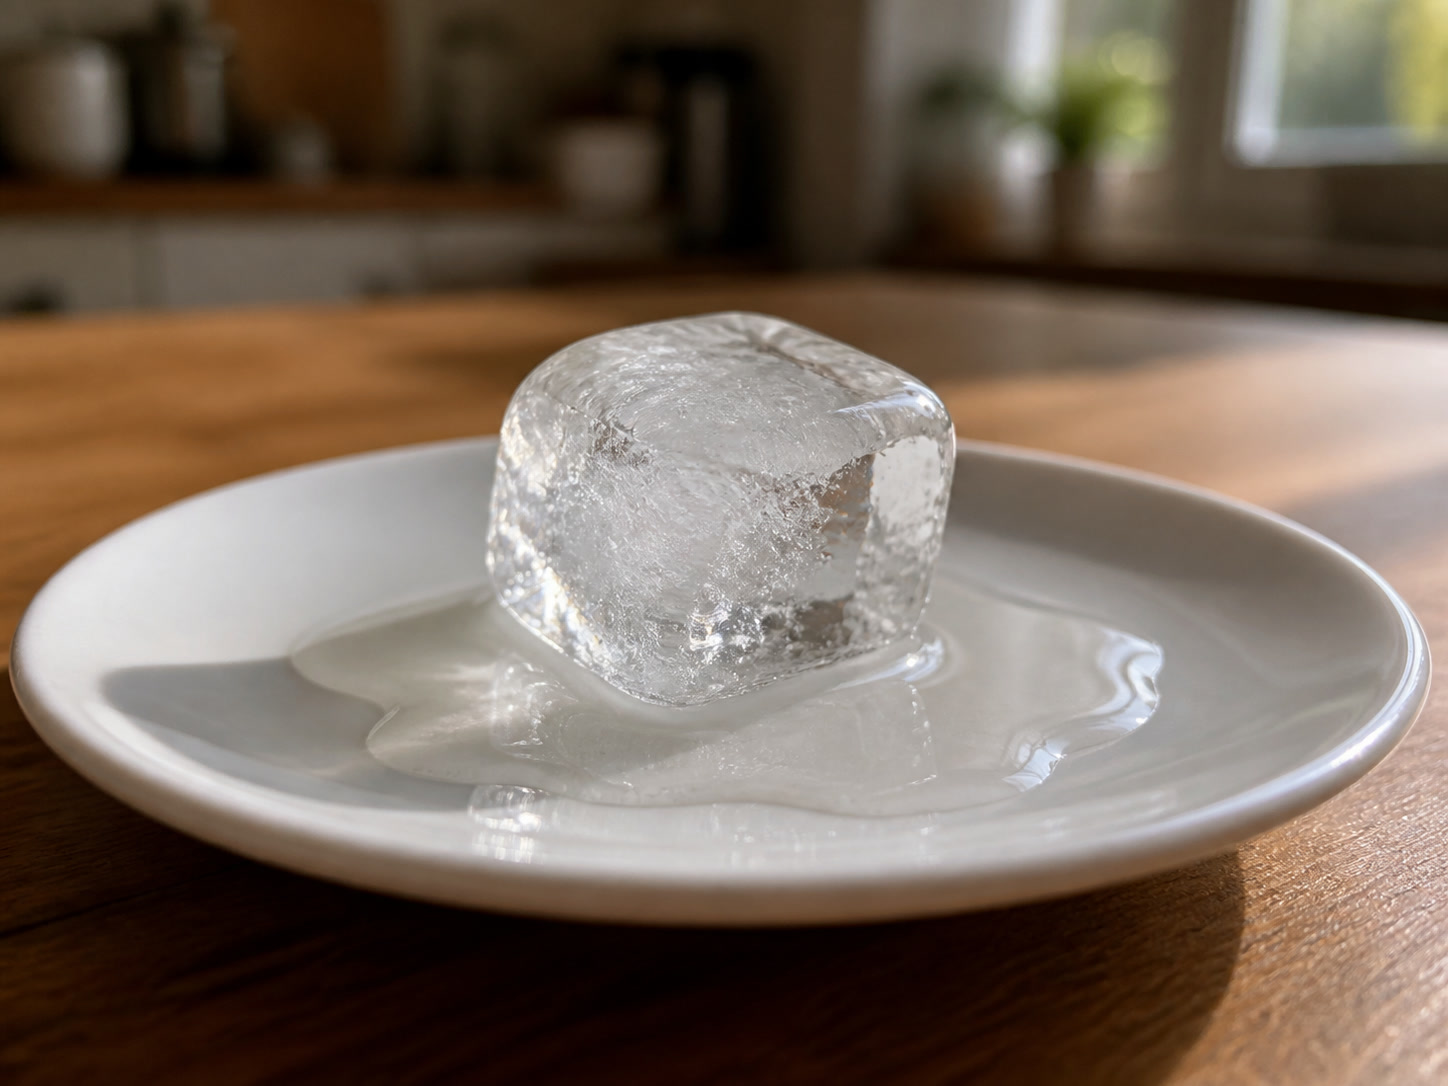
\includegraphics[width=0.52\linewidth]{images/book1/ai/g1-hot-cold-melting-cube.jpg}

{\small 温暖正在起作用：厨房里的冰块刚刚开始熔化成一摊水。}
\end{omfigure}

\begin{example}[寒冷也能获胜]\label{ex:g1:hot-and-cold:freezer}
冷冻室的作用恰恰相反：晚上在里面放一小杯水，
第二天早上你会发现它硬得像石头——
冰。温暖使冰熔化成水；强烈的寒冷则使水重新变成
冰。水会像这样不断地来回变化，
贯穿全书。
\end{example}

\section{练习}

\begin{exercise}[$\star$]\label{exo:g1:hot-and-cold:1}
按从冷到热排序：洗澡水；\ 一块冰块；\ 刚
出锅的汤；\ 你卧室里的空气。
\end{exercise}

\begin{exercise}[$\star$]\label{exo:g1:hot-and-cold:2}
找出合适的比较词：自来水与热巧克力相比是\dots\ 的，
但与从冰箱里拿出来的
橙汁相比是\dots\ 的。
\end{exercise}

\begin{exercise}[$\star$]\label{exo:g1:hot-and-cold:3}
说出四样能使周围物体变暖的东西。哪一样
能使整个公园变暖？
\end{exercise}

\begin{exercise}[$\star$]\label{exo:g1:hot-and-cold:4}
双手快速搓一搓，同时数到 $10$，然后摸一摸你的
脸颊。你感觉到了什么？搓手起了什么作用？
\end{exercise}

\begin{exercise}[$\star$]\label{exo:g1:hot-and-cold:5}
两块冰块一起从冷冻室拿出来。一块放在阳光下的盘子里，
另一块放在树荫下的盘子里。哪一块先熔化，
为什么？
\end{exercise}

\begin{exercise}[$\star$]\label{exo:g1:hot-and-cold:6}
冰块熔化后，盘子上留下的一摊水里有什么？
那块坚硬的冰去了哪里？
\end{exercise}

\begin{exercise}[$\star$]\label{exo:g1:hot-and-cold:7}
一个金属滑梯和一条木长椅整个上午都待在树荫里。汤姆
分别摸了摸两者，并说滑梯更冷。请用
请用\cref{rem:g1:hot-and-cold:fooled}解释实际发生的情况。
\end{exercise}

\begin{exercise}[$\star$]\label{exo:g1:hot-and-cold:8}
利用\cref{met:g1:hot-and-cold:compare}，说明如何判断
两碗水中哪一碗更暖和。为什么两次都要用同一只
手来摸？
\end{exercise}

\begin{exercise}[$\star\star$]\label{exo:g1:hot-and-cold:9}
莉亚堆了一个雪人，心疼它，就用自己的
暖和的外套把它裹了起来。她的弟弟说，外套会让雪人融化得更快；莉亚说
外套会让雪人在更长时间里保持寒冷。谁说得对？为什么？（可参考
\cref{rem:g1:hot-and-cold:coat}：衣服到底起什么作用？）
\end{exercise}
